\documentclass[12pt]{article}
\usepackage[margin=1in]{geometry}
\usepackage{newtxtext,newtxmath}
\usepackage{setspace}
\usepackage{hyperref}
\usepackage{tikz}
\usepackage{float}
\usetikzlibrary{arrows.meta,positioning,shapes.geometric,calc,decorations.pathreplacing}

% Brand colors
\definecolor{garnet}{HTML}{73000A}
\definecolor{atlantic}{HTML}{466A9F}
\definecolor{congaree}{HTML}{1F414D}
\definecolor{horseshoe}{HTML}{65780B}
\definecolor{rose}{HTML}{CC2E40}
\definecolor{honeycomb}{HTML}{A49137}
\definecolor{warmgrey}{HTML}{676156}
\definecolor{black90}{HTML}{363636}
\definecolor{black70}{HTML}{5C5C5C}
\definecolor{black50}{HTML}{A2A2A2}
\definecolor{black30}{HTML}{C7C7C7}
\definecolor{black10}{HTML}{ECECEC}
\definecolor{sandstorm}{HTML}{FFF2E3}

\author{J.C. Vaught}
\title{What Is Writing? A Contrastive Synthesis of Major Theories of Composition}
\date{}

\begin{document}

\maketitle

\begin{abstract}
This paper traces the intellectual trajectory of writing theory from Current-Traditional Rhetoric through Activity Theory, examining how each framework answers three foundational questions: What is writing? What makes writing good? How should writing be taught? Rather than declaring a single winner, the analysis identifies key axes of disagreement---product versus process versus activity, individual versus social, universal versus situated, writer-centered versus reader-centered, ideology-neutral versus ideology-aware, and theoretical versus practical---to understand what each theory illuminates and what it obscures. The paper concludes that the most productive understanding of writing emerges not from choosing among theories but from holding them in productive tension, while recognizing that writing is fundamentally social and that it constitutes the very contexts it addresses.
\end{abstract}

\section{Introduction}

What is writing? What makes writing good? How should writing be taught? These three questions---deceptively simple in their phrasing---have generated over a century of theoretical contestation within rhetoric and composition studies. The answers that different traditions have offered reveal not merely disagreements about pedagogy but fundamental divergences in epistemology, ontology, and ideology. A theory of writing is, inescapably, a theory of knowledge, selfhood, and social life.

This paper traces the intellectual trajectory from Current-Traditional Rhetoric through Expressivism, Cognitive Process Theory, Social-Epistemic Rhetoric, Rhetorical Genre Studies, Post-Process Theory, and Activity Theory, examining how each framework answers those three foundational questions and how each emerged, in significant part, as a corrective to the perceived failures of its predecessors. It then considers the practitioner's synthesis offered by Lawrence McEnerney, whose Reader-Value Model draws on multiple theoretical traditions to produce what may be the most widely consumed statement on academic writing in history. Throughout, the analysis is organized not as a sequential survey of theories but as a contrastive mapping along several axes of disagreement that cut across the chronological narrative: product versus process versus activity, individual versus social, universal versus situated, writer-centered versus reader-centered, ideology-neutral versus ideology-aware, and theoretical versus practical. The goal is not to declare a winner but to understand what each theory illuminates and what it obscures, and to identify the composite vision of writing that emerges when the full landscape is held in view.

\section{The Eight Theories at a Glance}

Before tracing the historical development and contrastive analysis of these theories, this section provides a brief overview of each framework and a visual model of its core commitments. Readers may refer back to these figures throughout the paper.

\subsection{Current-Traditional Rhetoric (1866--)}

Current-Traditional Rhetoric, codified by Alexander Bain and institutionalized at Harvard by Adams Sherman Hill, treats writing as the linear transcription of pre-formed thought into correct prose. The writer thinks first, then writes; the product is evaluated on grammar, paragraph unity, and conformity to prescribed modes of discourse. Invention---the generation of ideas---plays no formal role. The five-paragraph essay is CTR's most enduring artifact.

%% ---- FIGURE: CTR MODEL ----
\begin{figure}[H]
\centering
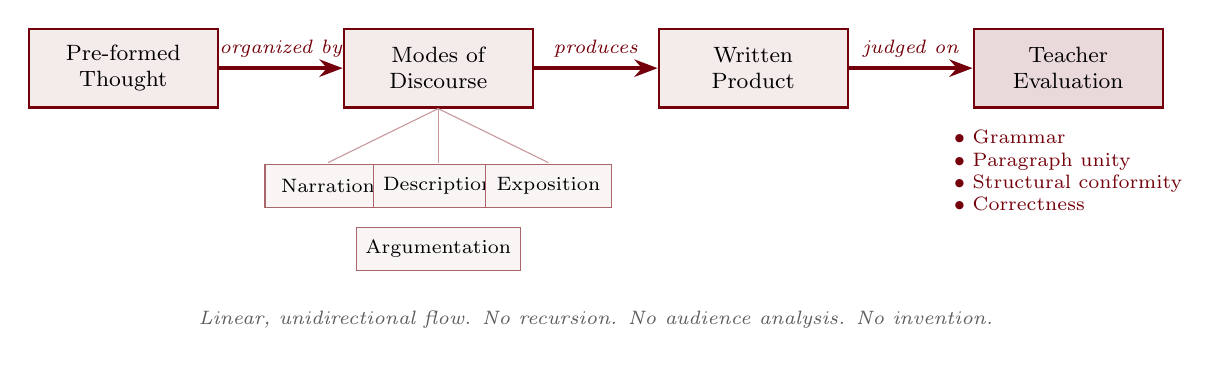
\begin{tikzpicture}[
    every node/.style={font=\footnotesize},
    box/.style={rectangle, draw=garnet, thick, fill=garnet!8,
        minimum width=2.4cm, minimum height=1cm, align=center, font=\footnotesize},
    modebox/.style={rectangle, draw=garnet!60, fill=garnet!4, minimum width=1.6cm,
        minimum height=0.55cm, align=center, font=\scriptsize},
]
% Main flow
\node[box] (thought) at (0,0) {Pre-formed\\Thought};
\node[box] (modes) at (4,0) {Modes of\\Discourse};
\node[box] (product) at (8,0) {Written\\Product};
\node[box, fill=garnet!15] (eval) at (12,0) {Teacher\\Evaluation};

\draw[-{Stealth}, very thick, garnet] (thought) -- (modes)
    node[midway, above, font=\scriptsize\itshape] {organized by};
\draw[-{Stealth}, very thick, garnet] (modes) -- (product)
    node[midway, above, font=\scriptsize\itshape] {produces};
\draw[-{Stealth}, very thick, garnet] (product) -- (eval)
    node[midway, above, font=\scriptsize\itshape] {judged on};

% Modes breakdown
\node[modebox] at (2.6,-1.5) {Narration};
\node[modebox] at (4,-1.5) {Description};
\node[modebox] at (5.4,-1.5) {Exposition};
\node[modebox] at (4,-2.3) {Argumentation};
\draw[thin, garnet!40] (modes.south) -- (2.6,-1.2);
\draw[thin, garnet!40] (modes.south) -- (4,-1.2);
\draw[thin, garnet!40] (modes.south) -- (5.4,-1.2);

% Evaluation criteria
\node[font=\scriptsize, text=garnet, align=left] at (12,-1.3) {
    $\bullet$ Grammar\\
    $\bullet$ Paragraph unity\\
    $\bullet$ Structural conformity\\
    $\bullet$ Correctness};

% Key annotation
\node[font=\scriptsize\itshape, text=black70, align=center] at (6, -3.2)
    {Linear, unidirectional flow. No recursion. No audience analysis. No invention.};
\end{tikzpicture}
\caption{\textbf{Current-Traditional Rhetoric.} Writing as linear transcription of pre-formed thought through prescribed modes into a product evaluated on surface correctness.}
\label{fig:ctr-model}
\end{figure}

\subsection{Expressivism (1966--)}

Expressivism, championed by Donald Murray, Ken Macrorie, and Peter Elbow, places the writer's authentic self at the center of the composing process. Writing is not transcription but discovery---writers do not know what they think until they have written it. Freewriting, peer workshops, and multiple drafts replace grammar drills and teacher-as-sole-evaluator. The goal is the cultivation of an authentic personal voice.

%% ---- FIGURE: EXPRESSIVISM MODEL ----
\begin{figure}[H]
\centering
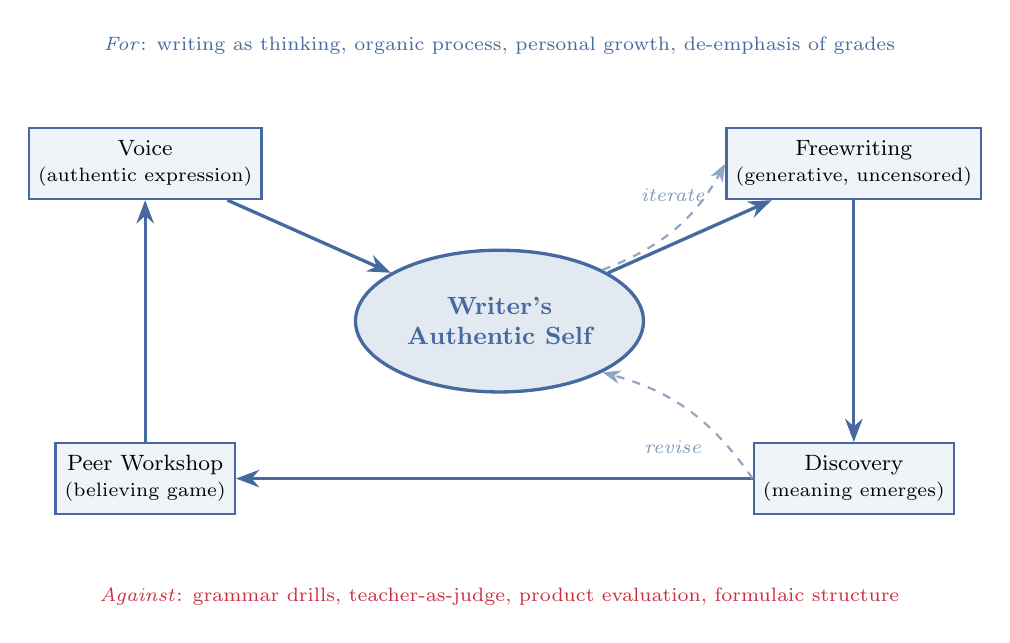
\begin{tikzpicture}[
    every node/.style={font=\footnotesize},
    box/.style={rectangle, draw=atlantic, thick, fill=atlantic!8,
        minimum width=2.2cm, minimum height=0.9cm, align=center, font=\footnotesize},
]
% Central writer
\node[ellipse, draw=atlantic, very thick, fill=atlantic!15,
    minimum width=3cm, minimum height=1.8cm, align=center, font=\small\bfseries,
    text=atlantic] (self) at (0,0) {Writer's\\Authentic Self};

% Surrounding process nodes in a cycle
\node[box] (free) at (4.5, 2) {Freewriting\\{\scriptsize (generative, uncensored)}};
\node[box] (discover) at (4.5, -2) {Discovery\\{\scriptsize (meaning emerges)}};
\node[box] (voice) at (-4.5, 2) {Voice\\{\scriptsize (authentic expression)}};
\node[box] (peer) at (-4.5, -2) {Peer Workshop\\{\scriptsize (believing game)}};

% Cycle arrows
\draw[-{Stealth}, very thick, atlantic] (self) -- (free);
\draw[-{Stealth}, very thick, atlantic] (free) -- (discover);
\draw[-{Stealth}, very thick, atlantic] (discover) -- (peer);
\draw[-{Stealth}, very thick, atlantic] (peer) -- (voice);
\draw[-{Stealth}, very thick, atlantic] (voice) -- (self);

% Revision spiral arrow
\draw[-{Stealth}, thick, atlantic!60, dashed] (discover.west) to[bend right=20] (self.south east);
\node[font=\scriptsize\itshape, text=atlantic!70] at (2.2, -1.6) {revise};

% Multiple drafts annotation
\draw[-{Stealth}, thick, atlantic!60, dashed] (self.north east) to[bend right=20] (free.west);
\node[font=\scriptsize\itshape, text=atlantic!70] at (2.2, 1.6) {iterate};

% Anti-CTR annotations
\node[font=\scriptsize, text=rose, align=center] at (0, -3.5)
    {\textit{Against}: grammar drills, teacher-as-judge, product evaluation, formulaic structure};
\node[font=\scriptsize, text=atlantic, align=center] at (0, 3.5)
    {\textit{For}: writing as thinking, organic process, personal growth, de-emphasis of grades};
\end{tikzpicture}
\caption{\textbf{Expressivism.} The writer's authentic self is the generative center. Writing proceeds through recursive cycles of freewriting, discovery, peer feedback, and voice cultivation.}
\label{fig:expressivism-model}
\end{figure}

\subsection{Cognitive Process Theory (1981)}

Linda Flower and John Hayes modeled writing as a recursive, goal-directed problem-solving process involving three major components---planning (generating, organizing, goal-setting), translating, and reviewing (evaluating, revising)---governed by a metacognitive monitor. Using think-aloud protocols, they demonstrated that expert writers deploy these processes hierarchically and non-linearly, in contrast to novice writers who follow more rigid, sequential patterns.

%% ---- FIGURE: COGNITIVE PROCESS MODEL ----
\begin{figure}[H]
\centering
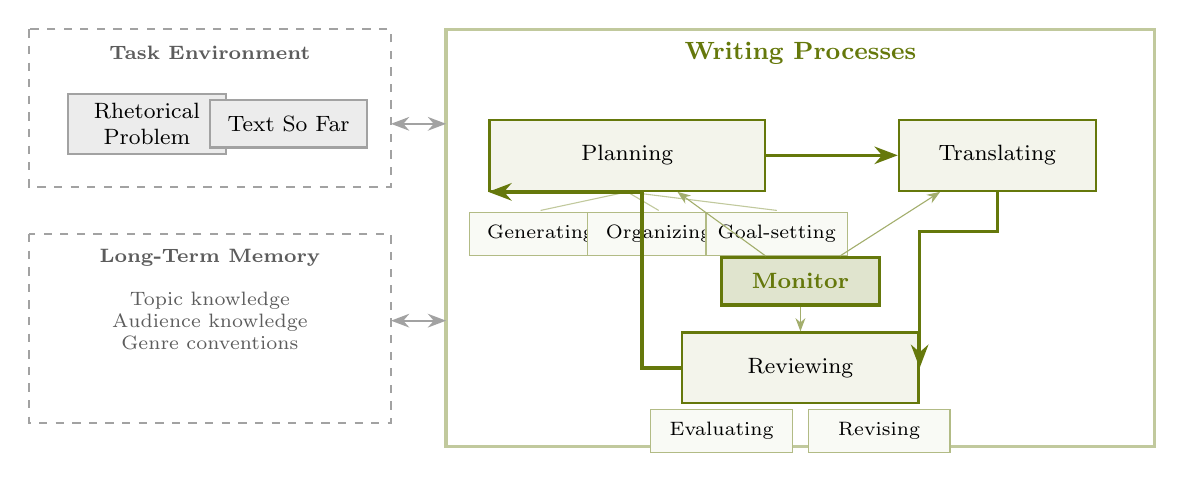
\begin{tikzpicture}[
    every node/.style={font=\footnotesize},
    box/.style={rectangle, draw=horseshoe, thick, fill=horseshoe!8,
        minimum width=2.5cm, minimum height=0.9cm, align=center, font=\footnotesize},
    subbox/.style={rectangle, draw=horseshoe!50, fill=horseshoe!4,
        minimum width=1.8cm, minimum height=0.55cm, align=center, font=\scriptsize},
    envbox/.style={rectangle, draw=black50, thick, fill=black10,
        minimum width=2.5cm, minimum height=0.9cm, align=center, font=\footnotesize},
]

% Task Environment
\draw[thick, black50, dashed] (-6.8, 3.8) rectangle (-2.2, 1.8);
\node[font=\scriptsize\bfseries, text=black70] at (-4.5, 3.5) {Task Environment};
\node[envbox, minimum width=2cm, minimum height=0.6cm] at (-5.3, 2.6) {Rhetorical\\Problem};
\node[envbox, minimum width=2cm, minimum height=0.6cm] at (-3.5, 2.6) {Text So Far};

% Long-Term Memory
\draw[thick, black50, dashed] (-6.8, 1.2) rectangle (-2.2, -1.2);
\node[font=\scriptsize\bfseries, text=black70] at (-4.5, 0.9) {Long-Term Memory};
\node[font=\scriptsize, text=black70, align=center] at (-4.5, 0.1) {Topic knowledge\\Audience knowledge\\Genre conventions};

% Writing Processes box
\draw[very thick, horseshoe!40] (-1.5, 3.8) rectangle (7.5, -1.5);
\node[font=\small\bfseries, text=horseshoe] at (3, 3.5) {Writing Processes};

% Planning
\node[box, minimum width=3.5cm] (plan) at (0.8, 2.2) {Planning};
\node[subbox] at (-0.3, 1.2) {Generating};
\node[subbox] at (1.2, 1.2) {Organizing};
\node[subbox] at (2.7, 1.2) {Goal-setting};
\draw[thin, horseshoe!40] (plan.south) -- (-0.3, 1.5);
\draw[thin, horseshoe!40] (plan.south) -- (1.2, 1.5);
\draw[thin, horseshoe!40] (plan.south) -- (2.7, 1.5);

% Translating
\node[box] (trans) at (5.5, 2.2) {Translating};

% Reviewing
\node[box, minimum width=3cm] (rev) at (3, -0.5) {Reviewing};
\node[subbox] at (2, -1.3) {Evaluating};
\node[subbox] at (4, -1.3) {Revising};

% Monitor
\node[rectangle, draw=horseshoe, very thick, fill=horseshoe!20,
    minimum width=2cm, minimum height=0.6cm, font=\footnotesize\bfseries,
    text=horseshoe] (mon) at (3, 0.6) {Monitor};

% Process arrows
\draw[-{Stealth}, very thick, horseshoe] (plan) -- (trans);
\draw[-{Stealth}, very thick, horseshoe] (trans.south) -- ++(0,-0.5) -| (rev.east);
\draw[-{Stealth}, very thick, horseshoe] (rev.west) -- ++(-0.5,0) |- (plan.south west);

% Monitor arrows
\draw[-{Stealth}, thin, horseshoe!60] (mon) -- (plan);
\draw[-{Stealth}, thin, horseshoe!60] (mon) -- (trans);
\draw[-{Stealth}, thin, horseshoe!60] (mon) -- (rev);

% Connections to environment and memory
\draw[{Stealth}-{Stealth}, thick, black50] (-2.2, 2.6) -- (-1.5, 2.6);
\draw[{Stealth}-{Stealth}, thick, black50] (-2.2, 0.1) -- (-1.5, 0.1);

\end{tikzpicture}
\caption{\textbf{Cognitive Process Theory (Flower \& Hayes, 1981).} Writing as recursive, hierarchically organized cognitive problem-solving. The task environment and long-term memory interact bidirectionally with all processes.}
\label{fig:cognitive-model}
\end{figure}

\subsection{Social-Epistemic Rhetoric (1987)}

James Berlin argued that all writing is ideological and that knowledge is socially constructed through discourse. Writer, material/social world, and language exist in a dialectical triad, each mutually constituting the others. CTR, expressivism, and cognitive rhetoric all disguise their ideological commitments; social-epistemic rhetoric makes ideology the explicit center of classroom activity, treating the composition classroom as an unavoidable site of political contestation.

%% ---- FIGURE: SOCIAL-EPISTEMIC MODEL ----
\begin{figure}[H]
\centering
\begin{tikzpicture}[
    every node/.style={font=\footnotesize},
    mainnode/.style={ellipse, draw=honeycomb, very thick, fill=honeycomb!10,
        minimum width=2.8cm, minimum height=1.4cm, align=center, font=\footnotesize},
]
% Central dialectic triangle
\node[mainnode] (writer) at (-4, -2) {Writer\\{\scriptsize (subject, constituted\\by discourse)}};
\node[mainnode] (world) at (4, -2) {Material/Social\\World};
\node[mainnode, fill=honeycomb!15] (language) at (0, 2.5) {Language\\{\scriptsize (agency of\\mediation)}};

% Dialectical arrows (bidirectional)
\draw[{Stealth}-{Stealth}, very thick, honeycomb] (writer) -- (world)
    node[midway, below, font=\scriptsize\itshape] {mutually constitutive};
\draw[{Stealth}-{Stealth}, very thick, honeycomb] (writer) -- (language)
    node[midway, left=0.1cm, font=\scriptsize\itshape, align=right] {shapes and\\is shaped by};
\draw[{Stealth}-{Stealth}, very thick, honeycomb] (world) -- (language)
    node[midway, right=0.1cm, font=\scriptsize\itshape, align=left] {constructs\\reality};

% Ideology permeating everything
\draw[very thick, rose, dashed] (0, 0.2) circle (4.2cm);
\node[font=\small\bfseries, text=rose] at (0, -4.8) {IDEOLOGY};
\node[font=\scriptsize\itshape, text=rose, align=center] at (0, -5.4)
    {permeates all elements; no rhetoric is ideologically neutral};

% Power/discourse annotations
\node[rectangle, draw=honeycomb!60, fill=sandstorm, font=\scriptsize, align=center,
    inner sep=3pt] at (5.5, 1) {Discourse\\communities};
\node[rectangle, draw=honeycomb!60, fill=sandstorm, font=\scriptsize, align=center,
    inner sep=3pt] at (-5.5, 1) {Power\\relations};

\draw[-{Stealth}, thin, honeycomb!60] (5.5, 0.6) -- (language);
\draw[-{Stealth}, thin, honeycomb!60] (-5.5, 0.6) -- (language);

\end{tikzpicture}
\caption{\textbf{Social-Epistemic Rhetoric (Berlin, 1988).} Writer, world, and language in dialectical relation, permeated by ideology. Language constructs rather than merely represents reality.}
\label{fig:social-epistemic-model}
\end{figure}

\subsection{Rhetorical Genre Studies (1984)}

Carolyn Miller redefined genres not as textual templates but as ``typified rhetorical actions based in recurrent situations.'' Charles Bazerman extended this insight through the concept of genre systems---interconnected documentary ecologies that constitute institutional activity. Genres are dynamic, historically evolving, and simultaneously enabling and constraining: they provide frameworks for action while reproducing community norms and power relations.

%% ---- FIGURE: RHETORICAL GENRE STUDIES MODEL ----
\begin{figure}[H]
\centering
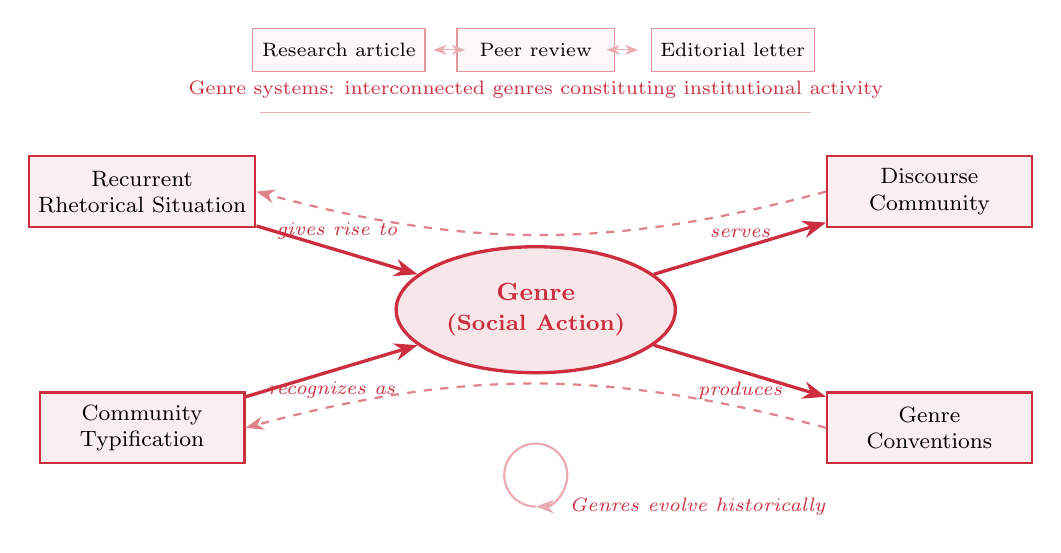
\begin{tikzpicture}[
    every node/.style={font=\footnotesize},
    box/.style={rectangle, draw=rose, thick, fill=rose!8,
        minimum width=2.6cm, minimum height=0.9cm, align=center, font=\footnotesize},
    smallbox/.style={rectangle, draw=rose!50, fill=rose!4,
        minimum width=2cm, minimum height=0.55cm, align=center, font=\scriptsize},
]

% Central concept
\node[ellipse, draw=rose, very thick, fill=rose!12,
    minimum width=3.2cm, minimum height=1.6cm, align=center,
    font=\small\bfseries, text=rose] (genre) at (0,0) {Genre\\{\footnotesize (Social Action)}};

% Recurrent situation
\node[box] (situation) at (-5, 1.5) {Recurrent\\Rhetorical Situation};
\node[box] (typify) at (-5, -1.5) {Community\\Typification};

% Community and conventions
\node[box] (community) at (5, 1.5) {Discourse\\Community};
\node[box] (conventions) at (5, -1.5) {Genre\\Conventions};

% Arrows
\draw[-{Stealth}, very thick, rose] (situation) -- (genre)
    node[midway, above, font=\scriptsize\itshape] {gives rise to};
\draw[-{Stealth}, very thick, rose] (typify) -- (genre)
    node[midway, below, font=\scriptsize\itshape] {recognizes as};
\draw[-{Stealth}, very thick, rose] (genre) -- (community)
    node[midway, above, font=\scriptsize\itshape] {serves};
\draw[-{Stealth}, very thick, rose] (genre) -- (conventions)
    node[midway, below, font=\scriptsize\itshape] {produces};

% Feedback loops
\draw[-{Stealth}, thick, rose!60, dashed] (conventions.west) to[bend right=15] (typify.east);
\draw[-{Stealth}, thick, rose!60, dashed] (community.west) to[bend left=15] (situation.east);

% Dynamic evolution
\draw[-{Stealth}, thick, rose!40] (0, -2.5) arc[start angle=-90, end angle=-450, radius=0.4]
    node[right=0.3cm, font=\scriptsize\itshape, text=rose] {Genres evolve historically};

% Genre system (Bazerman)
\node[font=\scriptsize, text=rose, align=center] at (0, 2.8)
    {Genre systems: interconnected genres constituting institutional activity};
\draw[thin, rose!40] (-3.5, 2.5) -- (3.5, 2.5);

% Examples
\node[smallbox] at (-2.5, 3.3) {Research article};
\node[smallbox] at (0, 3.3) {Peer review};
\node[smallbox] at (2.5, 3.3) {Editorial letter};
\draw[{Stealth}-{Stealth}, thin, rose!40] (-1.3, 3.3) -- (-0.9, 3.3);
\draw[{Stealth}-{Stealth}, thin, rose!40] (0.9, 3.3) -- (1.3, 3.3);

\end{tikzpicture}
\caption{\textbf{Rhetorical Genre Studies (Miller, 1984; Bazerman, 1994).} Genres as typified social actions arising from recurrent situations, serving and shaped by discourse communities.}
\label{fig:genre-model}
\end{figure}

\subsection{Post-Process Theory (1999)}

Thomas Kent, drawing on Donald Davidson's hermeneutic philosophy, argued that writing is public, interpretive, and situated---and therefore cannot be captured by any generalizable model. Communication proceeds through ``hermeneutic guessing'' rather than codifiable rules: writer and reader each bring prior interpretive theories that are adjusted in real time. Post-process theory offers not a new model but a principled refusal of all models.

%% ---- FIGURE: POST-PROCESS THEORY MODEL ----
\begin{figure}[H]
\centering
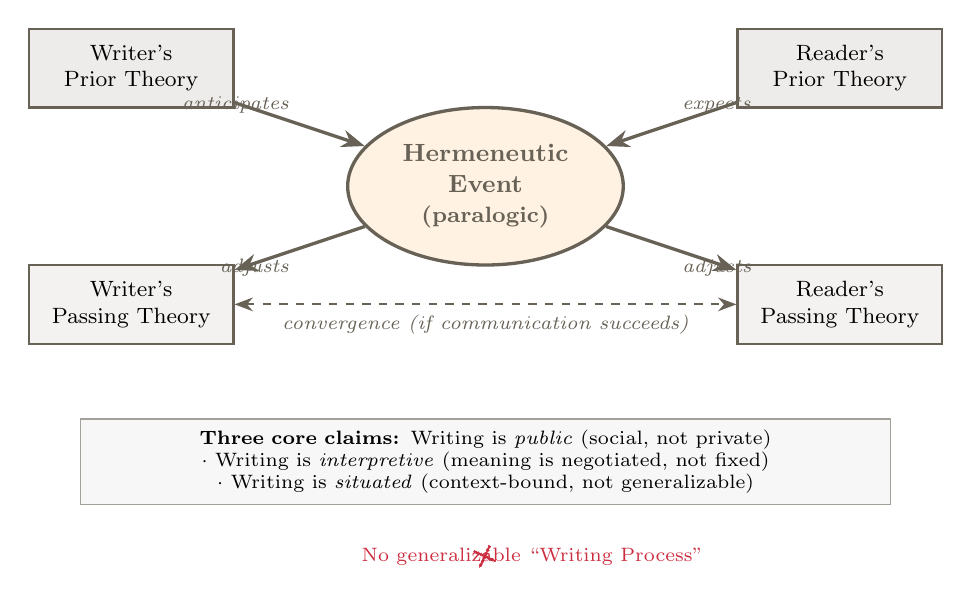
\begin{tikzpicture}[
    every node/.style={font=\footnotesize},
    box/.style={rectangle, draw=warmgrey, thick, fill=warmgrey!8,
        minimum width=2.6cm, minimum height=1cm, align=center, font=\footnotesize},
]

% Writer side
\node[box, fill=warmgrey!12] (wprior) at (-4.5, 2) {Writer's\\Prior Theory};
\node[box] (wpassing) at (-4.5, -1) {Writer's\\Passing Theory};

% Reader side
\node[box, fill=warmgrey!12] (rprior) at (4.5, 2) {Reader's\\Prior Theory};
\node[box] (rpassing) at (4.5, -1) {Reader's\\Passing Theory};

% Central hermeneutic event
\node[ellipse, draw=warmgrey, very thick, fill=sandstorm,
    minimum width=3.5cm, minimum height=2cm, align=center,
    font=\small\bfseries, text=warmgrey] (event) at (0, 0.5) {Hermeneutic\\Event\\{\footnotesize (paralogic)}};

% Arrows from prior to passing through event
\draw[-{Stealth}, very thick, warmgrey] (wprior) -- (event)
    node[midway, above left, font=\scriptsize\itshape] {anticipates};
\draw[-{Stealth}, very thick, warmgrey] (rprior) -- (event)
    node[midway, above right, font=\scriptsize\itshape] {expects};
\draw[-{Stealth}, very thick, warmgrey] (event) -- (wpassing)
    node[midway, below left, font=\scriptsize\itshape] {adjusts};
\draw[-{Stealth}, very thick, warmgrey] (event) -- (rpassing)
    node[midway, below right, font=\scriptsize\itshape] {adjusts};

% Convergence zone
\draw[{Stealth}-{Stealth}, thick, warmgrey, dashed] (wpassing) -- (rpassing)
    node[midway, below, font=\scriptsize\itshape] {convergence (if communication succeeds)};

% Three core claims
\node[rectangle, draw=warmgrey!60, fill=warmgrey!5, inner sep=4pt,
    font=\scriptsize, align=center, text width=10cm] at (0, -3)
    {\textbf{Three core claims:} Writing is \textit{public} (social, not private) $\cdot$
    Writing is \textit{interpretive} (meaning is negotiated, not fixed) $\cdot$
    Writing is \textit{situated} (context-bound, not generalizable)};

% X through "Process" label
\node[font=\large, text=rose, rotate=20] at (0, -4.2) {\sffamily\bfseries \texttimes};
\node[font=\scriptsize, text=rose] at (0.6, -4.2) {No generalizable ``Writing Process''};

\end{tikzpicture}
\caption{\textbf{Post-Process Theory (Kent, 1993, 1999).} Communication as paralogic hermeneutic event. Writer and reader adjust prior theories into passing theories through interpretive guessing, not codifiable rules.}
\label{fig:postprocess-model}
\end{figure}

\subsection{Activity Theory (1987)}

Rooted in Vygotsky's cultural-historical psychology and expanded by Engestr\"{o}m into a systems framework, activity theory models writing as a mediating tool within collectively organized activity systems. David Russell synthesized this framework with Bazerman's genre theory, demonstrating that writing can only be understood in relation to the full system---subject, object, mediating artifacts, rules, community, and division of labor---in which it operates. Contradictions between elements drive systemic change.

%% ---- FIGURE: ACTIVITY THEORY MODEL ----
\begin{figure}[H]
\centering
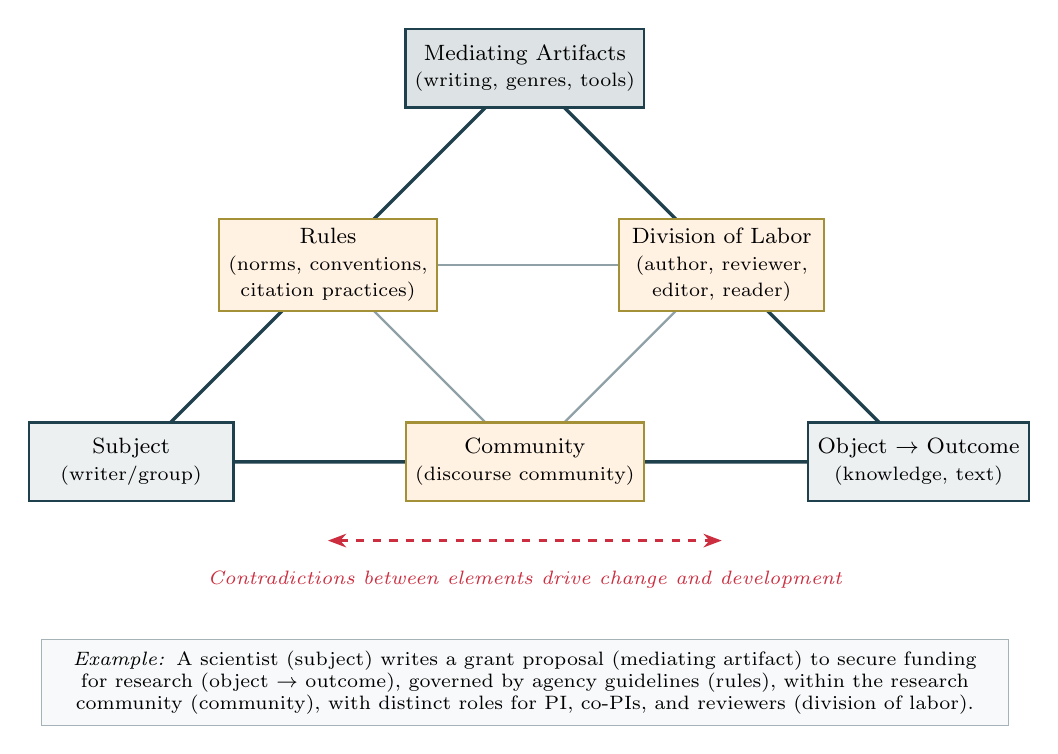
\begin{tikzpicture}[
    every node/.style={font=\footnotesize},
    element/.style={rectangle, draw=congaree, thick, fill=congaree!8,
        minimum width=2.6cm, minimum height=1cm, align=center, font=\footnotesize},
]

% Triangle vertices
\coordinate (top) at (0, 5);
\coordinate (left) at (-5, 0);
\coordinate (right) at (5, 0);

% Triangle edges
\draw[very thick, congaree] (top) -- (left) -- (right) -- cycle;

% Midpoints for lower triangle
\coordinate (midleft) at (-2.5, 2.5);
\coordinate (midright) at (2.5, 2.5);
\coordinate (midbottom) at (0, 0);

% Lower triangle lines
\draw[thick, congaree!50] (midleft) -- (midright);
\draw[thick, congaree!50] (midleft) -- (midbottom);
\draw[thick, congaree!50] (midright) -- (midbottom);

% Nodes at vertices
\node[element, fill=congaree!15] at (top) {Mediating Artifacts\\{\scriptsize (writing, genres, tools)}};
\node[element] at (left) {Subject\\{\scriptsize (writer/group)}};
\node[element] at (right) {Object $\rightarrow$ Outcome\\{\scriptsize (knowledge, text)}};

% Nodes at midpoints
\node[element, fill=sandstorm, draw=honeycomb] at (midbottom)
    {Community\\{\scriptsize (discourse community)}};
\node[element, fill=sandstorm, draw=honeycomb] at (midleft)
    {Rules\\{\scriptsize (norms, conventions,}\\{\scriptsize citation practices)}};
\node[element, fill=sandstorm, draw=honeycomb] at (midright)
    {Division of Labor\\{\scriptsize (author, reviewer,}\\{\scriptsize editor, reader)}};

% Contradictions annotation
\node[font=\scriptsize\itshape, text=rose, align=center] at (0, -1.5)
    {Contradictions between elements drive change and development};
\draw[thick, rose, dashed, {Stealth}-{Stealth}] (-2.5, -1) -- (2.5, -1);

% Example annotation
\node[rectangle, draw=congaree!40, fill=congaree!3, inner sep=4pt,
    font=\scriptsize, align=center, text width=12cm] at (0, -2.8)
    {\textit{Example:} A scientist (subject) writes a grant proposal (mediating artifact) to secure funding for research (object $\rightarrow$ outcome), governed by agency guidelines (rules), within the research community (community), with distinct roles for PI, co-PIs, and reviewers (division of labor).};

\end{tikzpicture}
\caption{\textbf{Activity Theory (Engestr\"{o}m, 1987; Russell, 1995, 1997).} Engestr\"{o}m's expanded activity system. Writing as mediating artifact within a collectively organized system of subject, object, rules, community, and division of labor.}
\label{fig:activity-model}
\end{figure}

\subsection{McEnerney's Reader-Value Model (2014)}

Lawrence McEnerney's framework inverts the orientation of traditional writing instruction: writing that is clear, organized, and correct may still fail entirely if it does not create \textit{value} for its readers. Value is defined not by the writer but by the discourse community, and the writer's first task is to understand what powerful readers in that community consider valuable. His practical techniques---opening with instability, studying community-specific value language, and revising for value rather than mere clarity---operationalize insights from genre theory and social-epistemic rhetoric into immediately actionable advice.

%% ---- FIGURE: MCENERNEY MODEL ----
\begin{figure}[H]
\centering
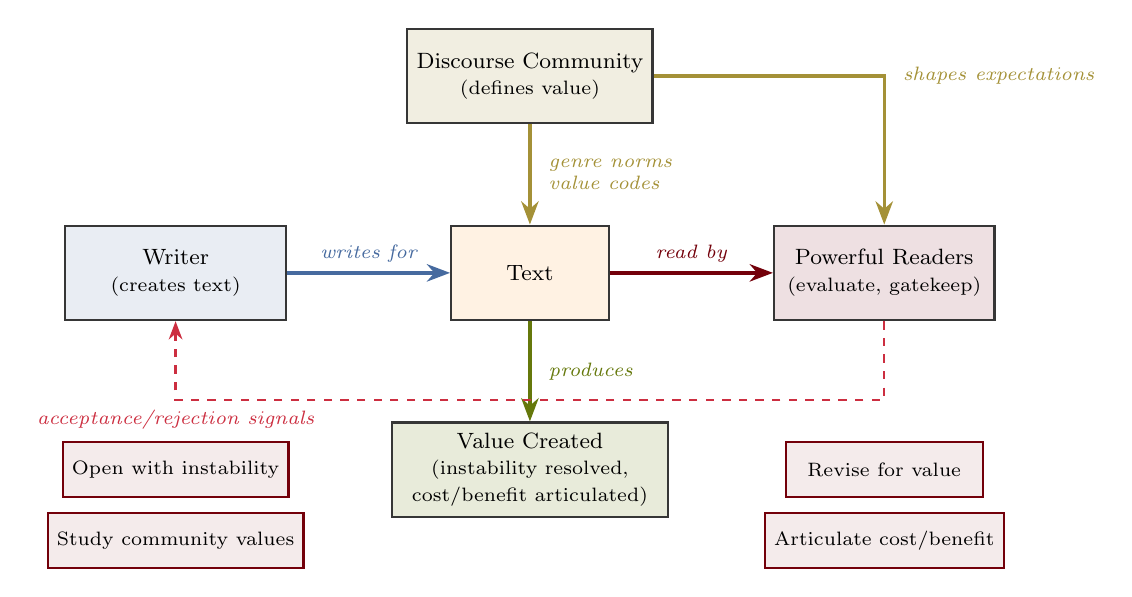
\begin{tikzpicture}[
    every node/.style={font=\footnotesize},
    mainbox/.style={rectangle, draw=black90, thick, minimum width=2.8cm,
        minimum height=1.2cm, align=center, font=\footnotesize},
    process/.style={rectangle, draw=garnet, thick, fill=garnet!8,
        minimum width=2.5cm, minimum height=0.7cm, align=center, font=\scriptsize},
]

% Writer
\node[mainbox, fill=atlantic!12] (writer) at (-4.5, 0) {Writer\\{\scriptsize (creates text)}};

% Discourse community
\node[mainbox, fill=honeycomb!15] (community) at (0, 2.5) {Discourse Community\\{\scriptsize (defines value)}};

% Readers
\node[mainbox, fill=garnet!12] (readers) at (4.5, 0) {Powerful Readers\\{\scriptsize (evaluate, gatekeep)}};

% Value
\node[mainbox, fill=horseshoe!15, minimum width=3.5cm] (value) at (0, -2.5)
    {Value Created\\{\scriptsize (instability resolved,}\\{\scriptsize cost/benefit articulated)}};

% Text in center
\node[mainbox, fill=sandstorm, minimum width=2cm] (text) at (0, 0) {Text};

% Arrows
\draw[-{Stealth}, very thick, atlantic] (writer) -- (text)
    node[midway, above, font=\scriptsize\itshape] {writes for};
\draw[-{Stealth}, very thick, garnet] (text) -- (readers)
    node[midway, above, font=\scriptsize\itshape] {read by};
\draw[-{Stealth}, very thick, honeycomb] (community) -- (text)
    node[midway, right=0.1cm, font=\scriptsize\itshape, align=left] {genre norms\\value codes};
\draw[-{Stealth}, very thick, honeycomb] (community.east) -| (readers.north)
    node[midway, right=0.1cm, font=\scriptsize\itshape] {shapes expectations};
\draw[-{Stealth}, very thick, horseshoe] (text) -- (value)
    node[midway, right=0.1cm, font=\scriptsize\itshape] {produces};

% Feedback loop from readers to writer
\draw[-{Stealth}, thick, rose, dashed] (readers.south) -- ++(0,-1) -| (writer.south)
    node[midway, below, font=\scriptsize\itshape] {acceptance/rejection signals};

% Key techniques annotations
\node[process] at (-4.5, -2.5) {Open with instability};
\node[process] at (-4.5, -3.4) {Study community values};
\node[process] at (4.5, -2.5) {Revise for value};
\node[process] at (4.5, -3.4) {Articulate cost/benefit};

\end{tikzpicture}
\caption{\textbf{McEnerney's Reader-Value Model (2014).} The writer creates text to produce value as defined by the discourse community. Powerful readers evaluate against community-specific value codes. Key techniques operationalize genre theory and social-epistemic rhetoric.}
\label{fig:mcenerney}
\end{figure}

\section{The Historical Arc: A Century of Correctives}

The history of writing theory from the late nineteenth century to the present is best understood not as linear progress toward truth but as a dialectical sequence in which each new framework arose from dissatisfaction with what came before. Current-Traditional Rhetoric (CTR), codified by Alexander Bain and institutionalized by Adams Sherman Hill at Harvard in the 1870s and 1880s, established the paradigm that would dominate American writing instruction for nearly a century. CTR treated writing as the transcription of pre-formed thought into correct prose, organized by the modes of discourse---narration, description, exposition, argumentation---and evaluated primarily on grammatical correctness, paragraph unity, and structural conformity. The five-paragraph essay, though not explicitly prescribed by Bain or Hill, became the paradigm's most recognizable artifact: a formula perfectly calibrated for standardized assessment, perfectly hostile to genuine inquiry.

Expressivism emerged in the late 1960s as a direct revolt against CTR's authoritarian formalism. Figures such as Donald Murray, Ken Macrorie, and Peter Elbow argued that writing is not transcription but discovery---that writers do not know what they think until they have written it. Where CTR placed the red pen at the center of instruction, expressivists placed the writer's authentic voice. Freewriting replaced grammar drills; peer workshops replaced the teacher-as-sole-evaluator; multiple drafts replaced the graded final product. The Dartmouth Conference of 1966, with its British emphasis on ``personal growth,'' provided institutional legitimacy for this reorientation.

Yet expressivism's celebration of the individual writer left a critical gap. If writing is self-discovery, what accounts for the systematic differences between expert and novice composing? Linda Flower and John Hayes, working from cognitive psychology at Carnegie Mellon, filled this gap with their Cognitive Process Theory (1981), which modeled writing as a recursive, goal-directed problem-solving process involving planning, translating, and reviewing, governed by a metacognitive monitor. Their think-aloud protocol methodology brought empirical rigor to a field that had relied largely on impressionistic observation. The Bereiter and Scardamalia (1987) distinction between knowledge-telling and knowledge-transforming extended the framework, demonstrating that expert writing involves a qualitatively different cognitive engagement with the composing task.

The Cognitive Process model (see Figure~\ref{fig:cognitive-model}), however, was almost immediately challenged for what it left out. Social-Epistemic Rhetoric, developed principally by James Berlin (1987, 1988) and supported by Patricia Bizzell's (1982) critique of cognitivism, argued that both CTR and the process theories---expressivist and cognitive alike---were ideologically complicit in ways they refused to acknowledge. Berlin contended that CTR presents itself as objective when it encodes a positivist epistemology; that expressivism claims to transcend ideology while reinforcing liberal individualism; and that cognitive rhetoric treats socially constructed conventions as the natural output of rational problem-solving. Against all three, Berlin advanced social-epistemic rhetoric, which holds that knowledge is socially constructed through discourse, that all writing is ideological, and that the composition classroom is unavoidably a site of political contestation.

Rhetorical Genre Studies (RGS), inaugurated by Carolyn Miller's ``Genre as Social Action'' (1984) and elaborated by Charles Bazerman and Amy Devitt, offered a more analytically precise framework for the social turn. Where Berlin dealt in ideology critique, Miller and her successors dealt in the concrete mechanisms by which communities organize their discursive practices. Genres, Miller argued, are not textual templates but ``typified rhetorical actions based in recurrent situations.'' Bazerman's concept of genre systems---the interconnected documentary ecologies that constitute institutional activity---provided tools for mapping how writing actually functions within social structures.

Post-Process Theory, crystallized by Thomas Kent's 1999 collection, pushed the critique of systematization to its logical extreme. Drawing on Donald Davidson's hermeneutic philosophy, Kent argued that writing is public, interpretive, and situated---and therefore cannot be captured by any generalizable model, including the Flower-Hayes process model. Gary Olson insisted that writing ``is not susceptible to systematization.'' Post-process theory offered not a new model but a principled refusal of all models: the claim that every act of writing is an unrepeatable hermeneutic event.

Activity Theory, rooted in Vygotsky's cultural-historical psychology and developed into a comprehensive systems framework by Engestrom (1987), provided what post-process theory conspicuously lacked: analytical apparatus. David Russell's (1995, 1997) application of activity theory to writing studies demonstrated that writing always functions as a mediating tool within larger activity systems characterized by subjects, objects, rules, communities, divisions of labor, and mediating artifacts. Russell's synthesis of activity theory with Bazerman's genre theory offered the field its most comprehensive framework for understanding writing as simultaneously individual and social, cognitive and material, textual and institutional.

\begin{figure}[H]
\centering
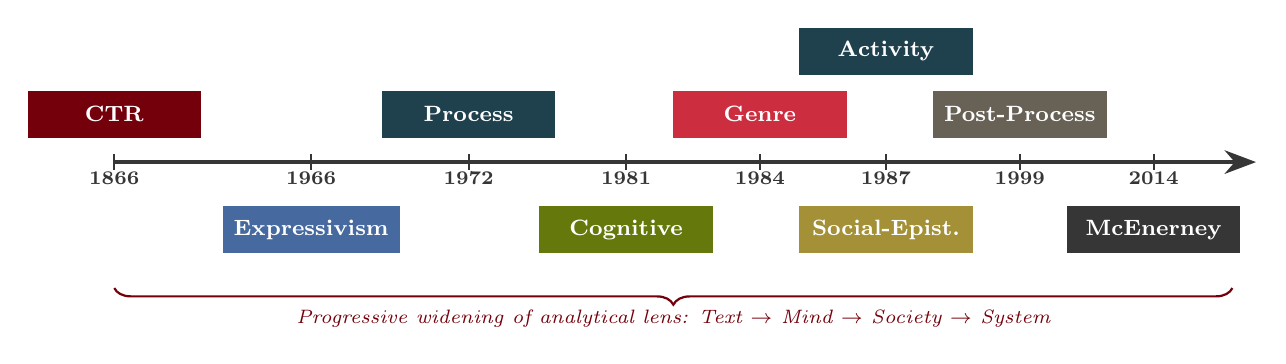
\begin{tikzpicture}[
    every node/.style={font=\footnotesize},
    yearnode/.style={font=\scriptsize\bfseries, text=black90},
    theorybox/.style={rectangle, minimum height=0.6cm, minimum width=2.2cm,
        text=white, font=\footnotesize\bfseries, inner sep=4pt},
]
% Timeline axis
\draw[very thick, black90, -{Stealth[length=4mm]}] (0,0) -- (14.5,0);
\node[yearnode, below] at (0,0) {1866};
\node[yearnode, below] at (2.5,0) {1966};
\node[yearnode, below] at (4.5,0) {1972};
\node[yearnode, below] at (6.5,0) {1981};
\node[yearnode, below] at (8.2,0) {1984};
\node[yearnode, below] at (9.8,0) {1987};
\node[yearnode, below] at (11.5,0) {1999};
\node[yearnode, below] at (13.2,0) {2014};

% Tick marks
\foreach \x in {0,2.5,4.5,6.5,8.2,9.8,11.5,13.2} {
    \draw[thick, black90] (\x,-0.1) -- (\x,0.1);
}

% Theory labels (alternating above/below)
\node[theorybox, fill=garnet, above=0.3cm] at (0,0) {CTR};
\node[theorybox, fill=atlantic, below=0.55cm] at (2.5,0) {Expressivism};
\node[theorybox, fill=congaree, above=0.3cm] at (4.5,0) {Process};
\node[theorybox, fill=horseshoe, below=0.55cm] at (6.5,0) {Cognitive};
\node[theorybox, fill=rose, above=0.3cm] at (8.2,0) {Genre};
\node[theorybox, fill=honeycomb, below=0.55cm] at (9.8,0) {Social-Epist.};
\node[theorybox, fill=warmgrey, above=0.3cm] at (11.5,0) {Post-Process};
\node[theorybox, fill=black90, below=0.55cm] at (13.2,0) {McEnerney};

% Activity Theory overlaps with Social-Epistemic
\node[theorybox, fill=congaree, above=1.1cm] at (9.8,0) {Activity};

% Widening lens annotation
\draw[decorate, decoration={brace, amplitude=6pt, mirror}, thick, garnet]
    (0,-1.6) -- (14.2,-1.6);
\node[font=\scriptsize\itshape, text=garnet, below=0.15cm] at (7.1,-1.6)
    {Progressive widening of analytical lens: Text $\rightarrow$ Mind $\rightarrow$ Society $\rightarrow$ System};

\end{tikzpicture}
\caption{Historical emergence of major writing theories. Each theory arose largely as a corrective to the perceived failures of its predecessors, progressively widening the unit of analysis from the text to the full activity system.}
\label{fig:timeline}
\end{figure}

This trajectory---from product to process to social practice to activity system---is not merely historical. It represents a progressive widening of the analytical lens: from the text alone (CTR), to the writer's mind (Expressivism, Cognitive Process), to the writer's social position (Social-Epistemic), to the community's genre conventions (RGS), to the irreducibility of the situated moment (Post-Process), to the full system of mediated social action (Activity Theory). Each widening corrected a genuine blindness in the preceding framework. Each also introduced new blindnesses of its own.

\section{Key Axes of Contrast}

\subsection{Product vs.\ Process vs.\ Activity}

The most fundamental axis of disagreement in writing theory concerns the proper object of attention. CTR is unapologetically product-oriented: the written text, evaluated against standards of correctness and formal propriety, is the alpha and omega of instruction. The process movement---encompassing both expressivism and cognitive process theory---shifted attention from the finished artifact to the composing activity that produces it. Murray's injunction to ``teach writing as a process not product'' (1972) became the movement's rallying cry. Yet even process theories retained the individual writer as the central unit of analysis; the ``process'' was something happening inside a person's head or at a person's desk.

Activity theory transcends this dichotomy by redefining writing as neither product nor process but as mediated social action within a system. The unit of analysis is not the text (CTR), not the writer's cognitive operations (Flower and Hayes), but the entire activity system---subject, object, mediating artifacts, rules, community, and division of labor. This reframing dissolves the product-process debate by showing that both the text and the composing process are analytically inseparable from the system of collective, tool-mediated activity that gives them meaning. A laboratory report is not merely a product to be evaluated or a process to be modeled; it is a mediating artifact through which the activity of scientific knowledge-production is carried out.

The practical consequence of this progression is significant. CTR asks: ``Does this text conform to standards?'' Process theories ask: ``Is the writer engaging in effective composing strategies?'' Activity theory asks: ``How does this writing function within the systems of human activity it mediates?'' Each question is legitimate, but the third subsumes the first two while adding dimensions they cannot reach.

\subsection{Individual vs.\ Social}

A second axis separates theories that locate writing in the individual mind from those that locate it in social systems. Expressivism and Cognitive Process Theory are both fundamentally individualist, though in different ways. Expressivism's individualism is romantic: the authentic self is the wellspring of good writing, and the writer's task is to discover and articulate that self despite the distorting pressures of institutional convention. Cognitive Process Theory's individualism is scientific: the composing process is modeled as a set of cognitive operations occurring within an individual mind, amenable to empirical study through think-aloud protocols.

Social-Epistemic Rhetoric and Activity Theory are both fundamentally social, though again in different ways. Berlin's social-epistemic framework emphasizes ideology and power: writing is a site where competing social interests are negotiated, and the individual writer is constituted through discourse and social interaction rather than existing prior to it. Activity Theory emphasizes systems and mediation: the individual writer is always a subject within an activity system, acting through culturally produced tools and embedded within communities, rules, and divisions of labor.

The individual-social tension has never been fully resolved, and the most productive work in the field occupies the space between these poles. Flower herself acknowledged the force of social critiques in her 1994 revision, \textit{The Construction of Negotiated Meaning}, which recast writing as a social-cognitive process in which meaning is negotiated among competing voices. Sondra Perl's (1980) concept of ``felt sense''---the pre-verbal, bodily experienced awareness that guides composing---reminds us that even the most socially situated writing passes through an embodied individual. The challenge is to theorize writing as simultaneously individual and social without collapsing one dimension into the other.

\begin{figure}[H]
\centering
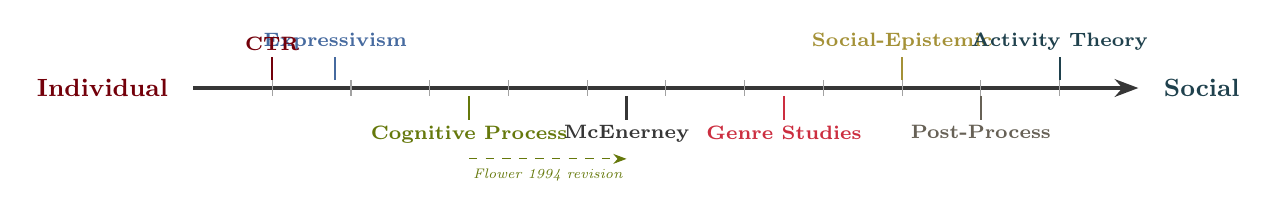
\begin{tikzpicture}[
    every node/.style={font=\footnotesize},
    theorymark/.style={font=\scriptsize\bfseries, inner sep=2pt},
]

% Individual vs Social axis
\draw[very thick, black90, -{Stealth[length=3mm]}] (-6,0) -- (6,0);
\node[font=\small\bfseries, text=garnet, anchor=east] at (-6.2,0) {Individual};
\node[font=\small\bfseries, text=congaree, anchor=west] at (6.2,0) {Social};

% Scale ticks
\foreach \x in {-5,-4,...,5} {
    \draw[black50] (\x,-0.1) -- (\x,0.1);
}

% Theory positions
\node[theorymark, text=atlantic, above=0.4cm] at (-4.2,0) {Expressivism};
\draw[thick, atlantic] (-4.2,0.1) -- (-4.2,0.4);

\node[theorymark, text=horseshoe, below=0.4cm] at (-2.5,0) {Cognitive Process};
\draw[thick, horseshoe] (-2.5,-0.1) -- (-2.5,-0.4);

\node[theorymark, text=garnet, above=0.4cm] at (-5,0) {CTR};
\draw[thick, garnet] (-5,0.1) -- (-5,0.4);

\node[theorymark, text=rose, below=0.4cm] at (1.5,0) {Genre Studies};
\draw[thick, rose] (1.5,-0.1) -- (1.5,-0.4);

\node[theorymark, text=honeycomb, above=0.4cm] at (3,0) {Social-Epistemic};
\draw[thick, honeycomb] (3,0.1) -- (3,0.4);

\node[theorymark, text=warmgrey, below=0.4cm] at (4,0) {Post-Process};
\draw[thick, warmgrey] (4,-0.1) -- (4,-0.4);

\node[theorymark, text=congaree, above=0.4cm] at (5,0) {Activity Theory};
\draw[thick, congaree] (5,0.1) -- (5,0.4);

\node[theorymark, text=black90, below=0.4cm] at (-0.5,0) {McEnerney};
\draw[thick, black90] (-0.5,-0.1) -- (-0.5,-0.4);

% Flower's revision arrow
\draw[-{Stealth}, thin, horseshoe, dashed] (-2.5,-0.9) -- (-0.5,-0.9);
\node[font=\tiny\itshape, text=horseshoe, below] at (-1.5,-0.9) {Flower 1994 revision};

\end{tikzpicture}
\caption{Positioning of writing theories along the individual--social axis. Theories on the left locate writing primarily in the individual mind or self; theories on the right locate it in social systems. Flower's 1994 revision (dashed arrow) shifted cognitive process theory toward the social pole.}
\label{fig:individual-social}
\end{figure}

\subsection{Universal vs.\ Situated}

Cognitive Process Theory aspired to universality: the Flower-Hayes model was presented as a description of the cognitive processes involved in composing, applicable in principle to all writers in all situations. Post-Process Theory denied this aspiration root and branch. Kent's Davidsonian framework insisted that every communicative act is a paralogic event---an unrepeatable hermeneutic encounter that cannot be captured by any codifiable system. Between these extremes, Rhetorical Genre Studies occupies an illuminating middle position. Genres are neither universal (they vary across communities and evolve historically) nor purely singular (they are, by definition, typified---recognizably recurrent responses to recognizably recurrent situations). Genre theory thus offers a way to talk about regularity in writing without claiming universality: there are patterns, but they are community-specific, historically contingent, and always subject to transformation.

Activity Theory similarly mediates between universality and situatedness. The activity system model is itself a universal analytical framework---it claims that all human activity has the same structural elements (subject, object, tools, rules, community, division of labor). But the specific content of any activity system is entirely situated: the rules, communities, tools, and objects of scientific writing differ from those of legal writing, which differ from those of journalism. The framework is universal; the writing is not. This distinction is philosophically important because it shows that post-process theory's rejection of universality may have been too sweeping. One can acknowledge that writing is always situated without concluding that nothing general can be said about it.

\subsection{Writer vs.\ Reader}

Perhaps the most practically consequential axis of contrast concerns orientation: is writing fundamentally about the writer or the reader? Expressivism is emphatically writer-centered. The purpose of writing is self-discovery; the writer's authentic voice is the standard of quality; the reader's role is to provide supportive, descriptive feedback that helps the writer develop. Elbow's believing game asks readers to enter sympathetically into the writer's vision rather than subjecting it to critical judgment.

McEnerney's Reader-Value Model inverts this orientation entirely. ``No one cares what is inside of your head,'' McEnerney declares. Good writing is writing that creates value for its readers, and value is defined not by the writer but by the discourse community in which the writing circulates. The writer's first task is not to express ideas but to understand what the target audience considers valuable. Rhetorical Genre Studies occupies a middle position: genres encode community expectations, so genre awareness equips the writer to calibrate their writing to their audience's conventions and values. But genre theory, unlike McEnerney, does not reduce the purpose of writing to the satisfaction of reader expectations; it also emphasizes that genres are sites of agency and contestation, not merely conformity.

\begin{figure}[H]
\centering

\begin{tikzpicture}[
    every node/.style={font=\footnotesize},
    theorymark/.style={font=\scriptsize\bfseries, inner sep=2pt},
]

% Writer vs Reader axis
\draw[very thick, black90, -{Stealth[length=3mm]}] (-6,0) -- (6,0);
\node[font=\small\bfseries, text=atlantic, anchor=east] at (-6.2,0) {Writer-Centered};
\node[font=\small\bfseries, text=garnet, anchor=west] at (6.2,0) {Reader-Centered};

% Scale ticks
\foreach \x in {-5,-4,...,5} {
    \draw[black50] (\x,-0.1) -- (\x,0.1);
}

% Theory positions
\node[theorymark, text=atlantic, above=0.4cm] at (-5,0) {Expressivism};
\draw[thick, atlantic] (-5,0.1) -- (-5,0.4);

\node[theorymark, text=horseshoe, below=0.4cm] at (-2,0) {Cognitive Process};
\draw[thick, horseshoe] (-2,-0.1) -- (-2,-0.4);

\node[theorymark, text=garnet, above=0.4cm] at (-3.5,0) {CTR};
\draw[thick, garnet] (-3.5,0.1) -- (-3.5,0.4);

\node[theorymark, text=rose, below=0.4cm] at (2,0) {Genre Studies};
\draw[thick, rose] (2,-0.1) -- (2,-0.4);

\node[theorymark, text=honeycomb, above=0.4cm] at (1,0) {Social-Epistemic};
\draw[thick, honeycomb] (1,0.1) -- (1,0.4);

\node[theorymark, text=warmgrey, below=0.4cm] at (-0.5,0) {Post-Process};
\draw[thick, warmgrey] (-0.5,-0.1) -- (-0.5,-0.4);

\node[theorymark, text=congaree, above=0.4cm] at (3,0) {Activity Theory};
\draw[thick, congaree] (3,0.1) -- (3,0.4);

\node[theorymark, text=black90, above=0.4cm] at (5,0) {\textbf{McEnerney}};
\draw[thick, black90] (5,0.1) -- (5,0.4);

\end{tikzpicture}
\caption{Positioning of writing theories along the writer--reader axis. Expressivism is emphatically writer-centered (writing as self-discovery), while McEnerney's Reader-Value Model is maximally reader-centered (``No one cares what is inside of your head''). Genre Studies and Activity Theory mediate between the poles by attending to community conventions and systems.}
\label{fig:writer-reader}
\end{figure}

The writer-reader tension illuminates a deeper question about the purpose of writing instruction. If writing is primarily about the writer---about self-discovery, cognitive development, and the cultivation of voice---then the composition classroom should be a space of personal growth. If writing is primarily about the reader---about creating value, meeting community standards, and achieving communicative effectiveness---then the classroom should be a space of socialization into discourse communities. Most practicing writing instructors would acknowledge that both purposes matter, but the theories they inherit push them toward one pole or the other.

\subsection{Ideology-Neutral vs.\ Ideology-Aware}

CTR, Expressivism, and Cognitive Process Theory all present themselves as ideologically neutral. CTR claims to teach the objective standards of correct English. Expressivism claims to liberate the authentic self from institutional constraint. Cognitive Process Theory claims to describe the universal architecture of composing. Berlin's central contribution was to demonstrate that all three are, in fact, deeply ideological. CTR's ``correct English'' encodes the linguistic norms of white, middle-class speakers. Expressivism's ``authentic self'' presupposes the romantic individualism of liberal capitalism. Cognitive Process Theory's ``rational problem-solver'' reflects a culturally specific construction of the autonomous agent.

Social-Epistemic Rhetoric's counter-claim---that it is ``self-consciously aware of its ideological stand''---raises a philosophical difficulty that Berlin never fully resolved. If all rhetoric is ideological, and if there is no non-ideological standpoint from which to evaluate competing rhetorical systems, then on what basis can social-epistemic rhetoric claim superiority? Berlin's answer---that self-conscious ideology is better than unconscious ideology because it provides mechanisms for self-critique---is plausible but not unanswerable. One might respond that the capacity for self-critique depends on intellectual honesty, not on theoretical framework, and that a self-described ideological approach risks becoming as dogmatic as the unconscious ideologies it critiques, precisely because it has inoculated itself in advance against charges of bias.

This tension between ideology-awareness and pedagogical neutrality remains unresolved in the field. Hairston's (1992) counterargument---that the social-epistemic classroom ``puts dogma before diversity, politics before craft''---articulates a genuine concern that ideological pedagogy can become indoctrination. The field has largely sided with Berlin in principle while remaining deeply ambivalent about the practical implications of his position.

\subsection{Theory vs.\ Practice}

A final axis separates theories that aspire to philosophical completeness from those that aspire to practical utility. Post-Process Theory is the most philosophically ambitious framework in composition studies. Its engagement with Davidsonian hermeneutics, its insistence on the irreducibility of communicative events, and its principled refusal of systematization represent a serious philosophical achievement. But its practical implications are notoriously thin. If writing cannot be systematized, what exactly should a writing teacher do on Monday morning? Post-process theorists have offered answers---mentoring, dialogue, situated practice---but these answers lack the operational specificity that classroom instruction demands.

McEnerney occupies the opposite pole. His Reader-Value Model is philosophically modest---he makes no claims about epistemology, ontology, or the nature of communicative interaction---but it is immediately actionable. Open with instability. Identify what your community values. Write for readers, not for yourself. Revise for value, not just for clarity. These directives can be implemented in a single writing session. The gap between post-process theory's philosophical depth and McEnerney's practical accessibility illuminates a persistent tension in writing studies between understanding writing and teaching it.

\section{McEnerney as Practitioner's Synthesis}

Lawrence McEnerney's Reader-Value Model deserves special attention not because it is the most theoretically sophisticated framework in the landscape---it is not---but because it achieves something that no purely academic theory has managed: a synthesis of insights from multiple traditions that is simultaneously rigorous and immediately usable.

Consider the intellectual genealogy. McEnerney's insistence that value is defined by discourse communities echoes the genre theory of Miller, Swales, and Bazerman, all of whom argue that texts derive their meaning and significance from the social contexts in which they circulate. His attention to power---his directive that writers must identify who holds evaluative authority within their community and understand what those powerful readers value---resonates directly with Berlin's social-epistemic rhetoric, which foregrounds the ideological and institutional dimensions of knowledge production. His rejection of writing as the transparent transmission of pre-existing thought aligns with the post-process insistence that writing is situated and interpretive. And his practical emphasis on instability language, cost-benefit framing, and community-specific value vocabulary operationalizes insights from genre analysis into concrete revision strategies.

What makes McEnerney's synthesis distinctive is its pragmatic orientation. Academic theories of writing tend to describe what writing is; McEnerney tells writers what to do about it. Genre theory explains that genres encode community values; McEnerney tells you to spend fifteen minutes a day reading published work in your field and circling the words that signal value. Social-epistemic rhetoric argues that discourse produces knowledge through social negotiation; McEnerney tells you to open with instability and articulate cost. Post-process theory insists that writing is irreducibly situated; McEnerney tells you to study the specific vocabulary of your target venue. In each case, the theoretical insight is preserved but translated into a concrete practice.

This translation comes at a cost, and the criticisms of the Reader-Value Model are serious. Its instrumentalism risks reducing writing to strategic calculation---a matter of identifying what powerful people want to hear and delivering it to them. Its emphasis on existing community values may reinforce hierarchies and exclude genuinely novel contributions that challenge prevailing standards. Its framework has little room for writing that is aesthetically motivated, personally expressive, or deliberately transgressive. And its advice to write what powerful readers value may function, for writers from marginalized backgrounds, as a mechanism of conformity rather than empowerment.

Yet these limitations do not diminish the fundamental achievement. McEnerney's viral lecture---viewed over eight million times---has reached more writers than every academic composition theory combined. The reason is not merely accessibility; it is that McEnerney addresses a question that academic theories tend to evade: given everything we know about writing as a social, situated, community-embedded activity, what should I actually do differently when I sit down to write? The practitioner's synthesis may lack the theoretical elegance of its academic sources, but it answers the question that writers actually ask.

\section{Contemporary Relevance: Toward a Composite Vision}

Which theories matter most today? The answer depends on the context, but a few observations can be made with confidence.

CTR, despite its intellectual bankruptcy as a theory of writing, remains the dominant paradigm in practice. The five-paragraph essay persists in secondary education. Standardized writing assessments reward correctness, organization, and formulaic structure. Style guides from Strunk and White to contemporary blog posts on ``good writing'' are overwhelmingly current-traditional in their assumptions. Any honest account of the field must acknowledge this gap between what composition scholars know and what actually happens in classrooms and testing centers.

Expressivism has been absorbed into the mainstream. Freewriting, peer workshops, multiple drafts, low-stakes writing, and the concept of ``voice'' are now pedagogical common sense, practiced even by instructors who would reject the expressivist label. The movement's central insight---that writing is a mode of thinking, not merely a mode of transmission---has become a foundational assumption of composition studies, contested by no one.

Cognitive Process Theory survives primarily in its methodology and its distinction between expert and novice composing. The specific flow-chart model of Flower and Hayes has been superseded, but the research tradition it inaugurated---empirical investigation of composing processes, attention to metacognition and self-regulation, the expert-novice paradigm---continues to inform educational psychology and cognitive science.

Social-Epistemic Rhetoric's influence is pervasive but diffuse. The field now takes for granted that writing is social, that discursive conventions are ideologically freighted, and that questions of power and access are legitimate concerns of composition pedagogy. These are Berlin's insights, even when his name is not invoked.

Genre Studies and Activity Theory provide the most productive analytical frameworks for current research. The synthesis of genre theory with activity theory---genres as tools within activity systems---offers the most comprehensive available account of how writing functions in disciplinary, professional, and institutional contexts. WAC and WID programs, now standard features of American higher education, rest on this theoretical foundation.

Post-Process Theory's legacy is primarily cautionary. Its insistence that writing resists systematization serves as a permanent check on the field's tendency to produce reductive models. Its philosophical depth enriches the discipline's self-understanding, even if its practical implications remain limited.

\begin{figure}[H]
\centering
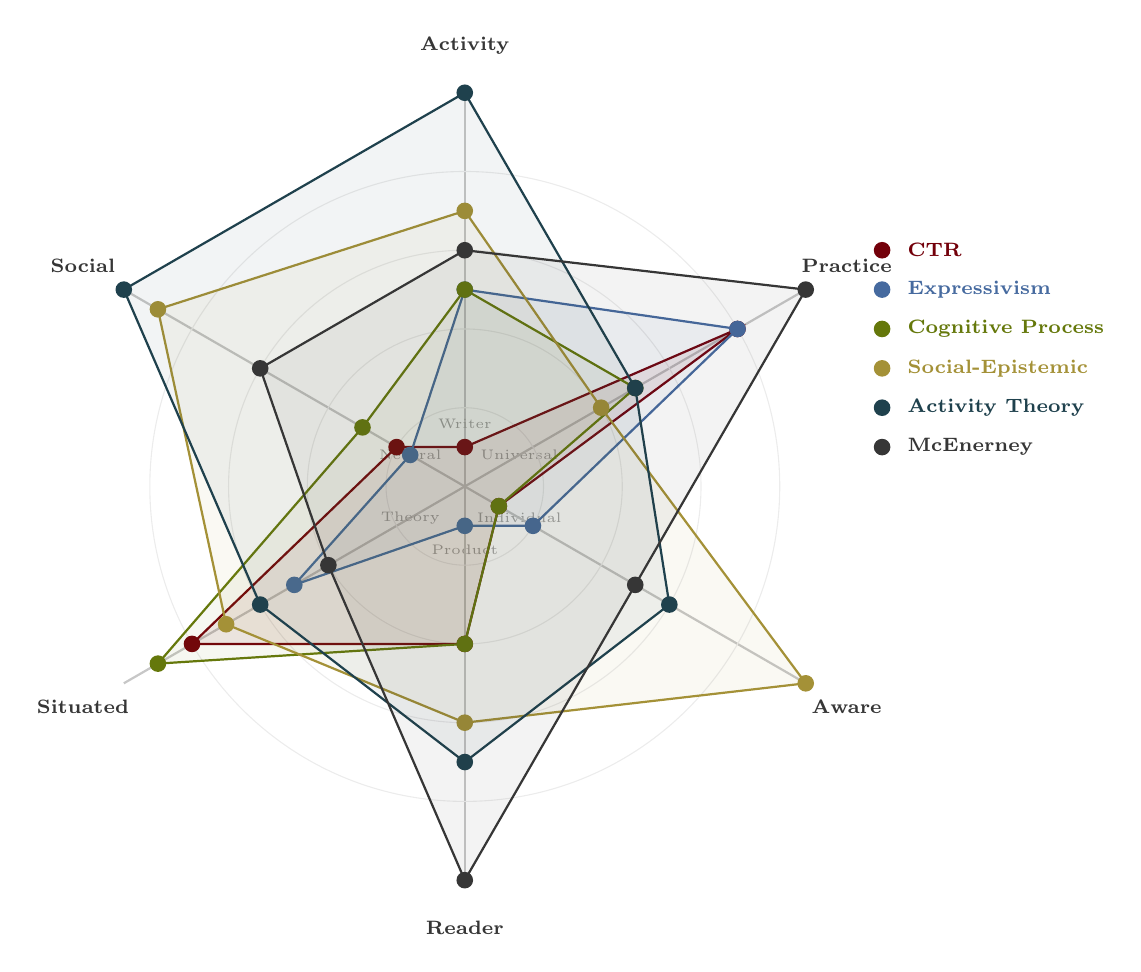
\begin{tikzpicture}[
    every node/.style={font=\scriptsize},
    axislabel/.style={font=\scriptsize\bfseries, text=black90},
    dot/.style={circle, inner sep=0pt, minimum size=6pt},
]

% Axes
\def\axislen{5.0}
\def\naxes{6}

% Axis labels and endpoints
\def\axes{
    {90/Product--Activity/Product/Activity},
    {150/Individual--Social/Individual/Social},
    {210/Universal--Situated/Universal/Situated},
    {270/Writer--Reader/Writer/Reader},
    {330/Ideology-Neutral--Aware/Neutral/Aware},
    {30/Theory--Practice/Theory/Practice}%
}

% Draw axes
\foreach \angle/\name/\labela/\labelb in \axes {
    \draw[thick, black30] (0,0) -- (\angle:\axislen);
    \node[axislabel] at (\angle:\axislen+0.6) {\labelb};
    % Inner label
    \node[font=\tiny, text=black50] at (\angle+180:0.8) {\labela};
}

% Grid circles
\foreach \r in {1,2,3,4} {
    \draw[thin, black10] (0,0) circle (\r cm);
}

% Helper macro: plot a theory as connected polygon
% Arguments: color, name, and 6 values (0-5 scale for each axis)
% Axis order: Product-Activity, Individual-Social, Universal-Situated,
%             Writer-Reader, Neutral-Aware, Theory-Practice

% CTR: product, individual, universal, writer-ish, neutral, practice
\draw[thick, garnet, fill=garnet, fill opacity=0.08]
    (90:0.5) -- (150:1) -- (210:4) -- (270:2) -- (330:0.5) -- (30:4) -- cycle;
\foreach \angle/\r in {90/0.5, 150/1, 210/4, 270/2, 330/0.5, 30/4} {
    \node[dot, fill=garnet] at (\angle:\r) {};
}

% Expressivism: process, individual, somewhat situated, writer, neutral, practice
\draw[thick, atlantic, fill=atlantic, fill opacity=0.06]
    (90:2.5) -- (150:0.8) -- (210:2.5) -- (270:0.5) -- (330:1) -- (30:4) -- cycle;
\foreach \angle/\r in {90/2.5, 150/0.8, 210/2.5, 270/0.5, 330/1, 30/4} {
    \node[dot, fill=atlantic] at (\angle:\r) {};
}

% Cognitive Process: process, individual, universal, balanced, neutral, balanced
\draw[thick, horseshoe, fill=horseshoe, fill opacity=0.06]
    (90:2.5) -- (150:1.5) -- (210:4.5) -- (270:2) -- (330:0.5) -- (30:2.5) -- cycle;
\foreach \angle/\r in {90/2.5, 150/1.5, 210/4.5, 270/2, 330/0.5, 30/2.5} {
    \node[dot, fill=horseshoe] at (\angle:\r) {};
}

% Social-Epistemic: activity, social, situated, balanced, very aware, theory
\draw[thick, honeycomb, fill=honeycomb, fill opacity=0.06]
    (90:3.5) -- (150:4.5) -- (210:3.5) -- (270:3) -- (330:5) -- (30:2) -- cycle;
\foreach \angle/\r in {90/3.5, 150/4.5, 210/3.5, 270/3, 330/5, 30/2} {
    \node[dot, fill=honeycomb] at (\angle:\r) {};
}

% Activity Theory: activity, social, both, balanced, moderate, moderate
\draw[thick, congaree, fill=congaree, fill opacity=0.06]
    (90:5) -- (150:5) -- (210:3) -- (270:3.5) -- (330:3) -- (30:2.5) -- cycle;
\foreach \angle/\r in {90/5, 150/5, 210/3, 270/3.5, 330/3, 30/2.5} {
    \node[dot, fill=congaree] at (\angle:\r) {};
}

% McEnerney: activity-ish, balanced, situated, reader, moderate, very practical
\draw[thick, black90, fill=black90, fill opacity=0.06]
    (90:3) -- (150:3) -- (210:2) -- (270:5) -- (330:2.5) -- (30:5) -- cycle;
\foreach \angle/\r in {90/3, 150/3, 210/2, 270/5, 330/2.5, 30/5} {
    \node[dot, fill=black90] at (\angle:\r) {};
}

% Legend
\node[font=\scriptsize\bfseries, text=garnet, anchor=west] at (5.5, 3.0) {CTR};
\node[font=\scriptsize\bfseries, text=atlantic, anchor=west] at (5.5, 2.5) {Expressivism};
\node[font=\scriptsize\bfseries, text=horseshoe, anchor=west] at (5.5, 2.0) {Cognitive Process};
\node[font=\scriptsize\bfseries, text=honeycomb, anchor=west] at (5.5, 1.5) {Social-Epistemic};
\node[font=\scriptsize\bfseries, text=congaree, anchor=west] at (5.5, 1.0) {Activity Theory};
\node[font=\scriptsize\bfseries, text=black90, anchor=west] at (5.5, 0.5) {McEnerney};

\foreach \y/\c in {3.0/garnet, 2.5/atlantic, 2.0/horseshoe, 1.5/honeycomb, 1.0/congaree, 0.5/black90} {
    \node[dot, fill=\c] at (5.3, \y) {};
}

\end{tikzpicture}
\caption{Radar chart comparing six major writing theories across the six axes of contrast identified in this paper. Each theory's ``footprint'' reflects its characteristic emphases. Outward position indicates stronger identification with the labeled pole (e.g., farther on the Activity axis means more activity-oriented; farther on the Reader axis means more reader-centered). Note that no single theory spans all dimensions equally, illustrating why a composite approach is necessary.}
\label{fig:radar}
\end{figure}

A ``best of all worlds'' approach to writing instruction would draw on all of these traditions. It would teach the formal conventions that CTR codified (because conventions matter in professional contexts) without treating them as the essence of good writing. It would use expressivist techniques---freewriting, journals, low-stakes writing---to build fluency and foster the experience of writing as thinking. It would draw on cognitive process research to help students develop sophisticated planning and revision strategies. It would engage students in the critical examination of discourse that social-epistemic rhetoric demands. It would cultivate genre awareness, teaching students to analyze the rhetorical situations and community conventions that shape writing in specific contexts. It would honor the post-process insight that every writing situation is unique, requiring adaptive rather than mechanical responses. And it would situate all of this within an activity-theoretic understanding of writing as tool-mediated social action embedded in systems of collective practice.

McEnerney's Reader-Value Model, for all its limitations, comes closest to achieving this synthesis in practice. Its emphasis on community-defined value incorporates genre theory's attention to discourse conventions. Its focus on reader needs incorporates audience awareness. Its instability framework provides a concrete heuristic for engaging with the rhetorical situation. And its insistence that the transition from student writing to professional writing requires a fundamental reconception of purpose echoes the activity-theoretic claim that writing can only be understood in relation to the activity systems it mediates.

\section{Conclusion: What the Trajectory Reveals}

The field's trajectory from CTR to Activity Theory reveals something important about the nature of writing itself. Writing is, irreducibly, all of the things that the various theories claim it is. It is a product, shaped by conventions and evaluated against standards. It is a process, involving recursive cognitive operations that unfold over time. It is an expression of individual identity and a site of self-discovery. It is a social act, embedded in discourse communities and shaped by relations of power. It is a genre-mediated response to recurrent rhetorical situations. It is an unrepeatable hermeneutic event, situated in a particular moment and context. It is a tool within an activity system, mediating between subjects and objects within communities governed by rules and divisions of labor. No single theory captures all of these dimensions, because writing is more complex than any single theory can accommodate.

The failure of the field to produce a unified theory of writing is not a failure at all. It is a reflection of the fact that writing---like language, like thought, like social life---is a phenomenon whose full complexity exceeds the grasp of any single analytical framework. The productive tension among competing theories is not a problem to be solved but a condition to be cultivated. Each theory illuminates aspects of writing that the others obscure. Each asks questions that the others cannot formulate. The richest understanding of writing comes not from choosing among theories but from holding them in productive tension, attending to what each reveals and remaining alert to what each conceals.

What the trajectory does reveal, with increasing clarity, is that writing is fundamentally social. Even the most individualist theories---expressivism, cognitive process theory---have been compelled to acknowledge the social dimensions of composing. Flower's 1994 revision incorporated social negotiation. Contemporary expressivist scholarship foregrounds discourse communities and cultural context. The direction of the field's evolution, from the isolated writer to the activity system, reflects a deepening recognition that writing does not merely occur in social contexts; it constitutes them. Writing produces the communities it addresses, the knowledge it claims to represent, and the identities of the writers who compose it. This insight---that writing is not a mirror held up to a pre-existing social world but a tool through which that world is continuously constructed---may be the single most important contribution of a century of theoretical inquiry.

\newpage

\section*{References}

Bain, A. (1866). \textit{English Composition and Rhetoric: A Manual}. Longmans, Green.

Bartholomae, D. (1986). Inventing the university. \textit{Journal of Basic Writing}, 5(1), 4--23.

Bazerman, C. (1988). \textit{Shaping Written Knowledge: The Genre and Activity of the Experimental Article in Science}. University of Wisconsin Press.

Bazerman, C. (1994). Systems of genres and the enactment of social intentions. In A. Freedman \& P. Medway (Eds.), \textit{Genre and the New Rhetoric} (pp. 79--101). Taylor \& Francis.

Bazerman, C., \& Russell, D. R. (Eds.). (2003). \textit{Writing Selves/Writing Societies: Research from Activity Perspectives}. The WAC Clearinghouse.

Bereiter, C., \& Scardamalia, M. (1987). Knowledge telling and knowledge transforming in written composition. In S. Rosenberg (Ed.), \textit{Advances in Applied Psycholinguistics, Volume 2} (pp. 142--175). Cambridge University Press.

Berlin, J. A. (1987). \textit{Rhetoric and Reality: Writing Instruction in American Colleges, 1900--1985}. Southern Illinois University Press.

Berlin, J. A. (1988). Rhetoric and ideology in the writing class. \textit{College English}, 50(5), 477--494.

Bizzell, P. (1982). Cognition, convention, and certainty: What we need to know about writing. \textit{PRE/TEXT}, 3(3), 213--243.

Connors, R. J. (1997). \textit{Composition-Rhetoric: Backgrounds, Theory, and Pedagogy}. University of Pittsburgh Press.

Devitt, A. J. (2004). \textit{Writing Genres}. Southern Illinois University Press.

Dobrin, S. I. (2011). \textit{Postcomposition}. Southern Illinois University Press.

Elbow, P. (1973). \textit{Writing Without Teachers}. Oxford University Press.

Elbow, P. (1981). \textit{Writing With Power: Techniques for Mastering the Writing Process}. Oxford University Press.

Engestrom, Y. (1987). \textit{Learning by Expanding: An Activity-Theoretical Approach to Developmental Research}. Orienta-Konsultit.

Flower, L. (1994). \textit{The Construction of Negotiated Meaning: A Social Cognitive Theory of Writing}. Southern Illinois University Press.

Flower, L., \& Hayes, J. R. (1981). A cognitive process theory of writing. \textit{College Composition and Communication}, 32(4), 365--387.

Graff, G., \& Birkenstein, C. (2006). \textit{``They Say / I Say'': The Moves That Matter in Academic Writing}. W. W. Norton.

Hairston, M. (1992). Diversity, ideology, and teaching writing. \textit{College Composition and Communication}, 43(2), 179--193.

Harris, J. (1997). \textit{A Teaching Subject: Composition Since 1966}. Prentice Hall.

Hayes, J. R. (1996). A new framework for understanding cognition and affect in writing. In C. M. Levy \& S. Ransdell (Eds.), \textit{The Science of Writing} (pp. 1--27). Lawrence Erlbaum.

Hill, A. S. (1878). \textit{The Principles of Rhetoric and Their Application}. Harper \& Brothers.

Kent, T. (1993). \textit{Paralogic Rhetoric: A Theory of Communicative Interaction}. Bucknell University Press.

Kent, T. (Ed.). (1999). \textit{Post-Process Theory: Beyond the Writing-Process Paradigm}. Southern Illinois University Press.

Macrorie, K. (1970). \textit{Telling Writing}. Hayden Book Company.

McEnerney, L. (2014). The craft of writing effectively [Video lecture]. University of Chicago Leadership Lab. Retrieved from https://www.youtube.com/watch?v=vtIzMaLkCaM

Miller, C. R. (1984). Genre as social action. \textit{Quarterly Journal of Speech}, 70(2), 151--167.

Murray, D. M. (1972). Teach writing as a process not product. \textit{The Leaflet}, 71(3), 11--14.

Olson, G. A. (1999). Toward a post-process composition: Abandoning the rhetoric of assertion. In T. Kent (Ed.), \textit{Post-Process Theory} (pp. 7--15). Southern Illinois University Press.

Perl, S. (1980). Understanding composing. \textit{College Composition and Communication}, 31(4), 363--369.

Russell, D. R. (1995). Activity theory and its implications for writing instruction. In J. Petraglia (Ed.), \textit{Reconceiving Writing, Rethinking Writing Instruction} (pp. 51--77). Lawrence Erlbaum.

Russell, D. R. (1997). Rethinking genre in school and society: An activity theory analysis. \textit{Written Communication}, 14(4), 504--554.

Swales, J. M. (1990). \textit{Genre Analysis: English in Academic and Research Settings}. Cambridge University Press.

Williams, J. M. (1990). \textit{Style: Toward Clarity and Grace}. University of Chicago Press.

\end{document}
